\subsection{Loan Application Process}
\label{subsec:loan-app-process}
\textit{Loan Application Process} dataset is synthetically created and consists of four variants of a simple loan application in a financial institute. These event logs are used to test different approaches of discovering a configurable process model from a collection of event logs \cite{buijs2014flexible}. In this dataset there are a total of 475 cases and 2440 events with a fairly even distribution between variants and these variants are used as organizational logs and the methodology presented in this thesis study is be applied.

\begin{itemize}
  \item In \textit{Process Model Mining} stage, process models resulted with perfect fitness and high appropriateness as it is expected from a synthetically generated dataset without noise.
  \item In \textit{Performance Indicator Analysis} stage, firstly event logs are replayed over process models and performance indicators are calculated and then organizations are clustered based on their performance indicators. In order to avoid overfitting,  with two clusters, Variant \#1, \#2, and \#4 are grouped into one cluster where only Variant \#3 is left to other cluster. 
  \item In \textit{Mismatch Pattern Analysis} stage, number of mismatch patterns are analyzed with the \textit{graph-edit similarity} between each two organization. As the similarity between process models decreases our method spots more mismatch patterns and it ensures that the developed mismatch pattern analyzers work as expected for this dataset. 
  \item In \textit{Recommendation Generation} stage, for different threshold values, number of performance indicators that are performing better for the selected organization and spotted mismatch patterns are plotted in Figure~\ref{fig:loan-recommendation-generation-analysis}. 
    \begin{figure}
    	\centering
    	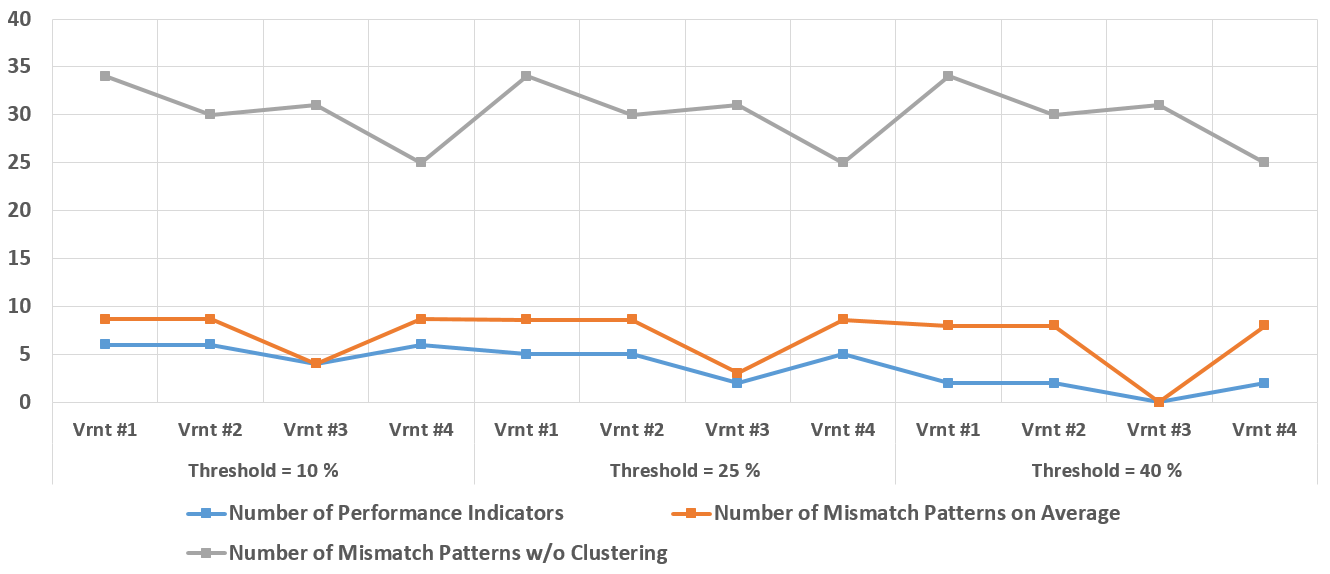
\includegraphics[width=\textwidth]{5_results_discussions/loan-application-process/recommendation-generation-analysis}
    	\caption{Recommendation Generation analysis for Loan Application Process dataset}
      \label{fig:loan-recommendation-generation-analysis}
    \end{figure}
  In order to construct the data in Figure~\ref{fig:loan-recommendation-generation-analysis}, every organization is selected one-by-one with different threshold values. For each analysis, number of performance indicators and average number of mismatch patterns causing them are plotted. In addition, total number of mismatch patterns without clustering is added as an upper bound. With the help of this upper bound, responsiveness and degree of helping the user to focus on the performance improvement can be analyzed. As can be seen, for each threshold value, average number of mismatch patterns \textit{with performance indicator clustering} are very low compared to \textit{without clustering}. In other words, when user wants to improve its performance with any threshold, there is significantly less number of mismatch patterns on average to check. This shows the methodology proposed in this study can help users to focus on differences between organizations given this dataset.
\end{itemize}